\chapter{Basics of C}
There are certain rules in every language, certain grammar which
dictates the
way language will be spoken and written. It has a script to write
using. Similarly, programming languages have BNF (Backus-Naur Form)
context-free grammar. There are valid characters in a programming language and
a set of keywords. There are constructs to handle control flow, loops
etc. There are facilities provided by language to deal with numbers and strings
separately, to reuse the code and some basic data structures to facilitate
programming. However, programming language rule-set is very small compared
to a natural programming language. Also, when using natural programming
language like talking to someone or writing something the other person can
understand your intent but in programming you cannot violate rules. The grammar
is context-free. Compilers or interpreters cannot deduce your intent by reading
code. They are not intelligent. You make a mistake and it will refuse to listen
to you no matter what you do. Therefore, it is very essential to understand
these rules very clearly and correctly.

\section{The C Character Set}
The following form the C character set you are allowed to use in it which is
given in \S(iso.5.2.1):

\begin{Verbatim}[frame=single]
[a-z] [A-Z] [0-9] ~ ! # % ^ & * ( ) - = [ ] \ ; ' , . / _ + { } | : " < > ?
\end{Verbatim}
\index{character set}

This means along with other symbols you can use all English alphabets (both
uppercase and lowercase) and Arabic numerals. Symbols like \texttt{\$} and
\texttt{@} are not part of C's character set. But strings can contain any
these characters also. Strings are sequence of characters with double quotes
and double quotes itself are escaped with \texttt{$\backslash$}. Also,
\texttt{\$} and \texttt{@} can also be value of characters. Characters are
values containing single characters withing single quotes. We will see more of
these in their individual sections. However, English is not the only
spoken language in the world. Therefore in other non-English speaking counties
there are keyboard where certain characters present in above set are not
present. The inventors of C were wise enough to envision this and provide the
facility in form of trigraph sequences. Given below is the trigraph sequence
table given in \S(iso.5.2.1.1):

\begin{table}[H]
 \begin{center}
 \caption{Trigraph Sequences}
\begin{tabular}{|c|c|c|c|c|c|}
\hline
\textbf{Trigraph}&\textbf{Equivalent}&\textbf{Trigraph}&\textbf{Equivalent}&\textbf{Trigraph}&\textbf{Equivalent}\\
\hline
??=&\#&??'&\textasciicircum&??!&|\\
\hline
??(&[&??)&]&??$<$&\{\\
\hline
??$>$&\}&??/&\textbackslash&??-&\textasciitilde\\
\hline
\end{tabular}
\end{center}
\end{table}
\index{trigraph sequences}

However, you should refrain from using trigraph sequences for portability 
reasons as suggested by GNU coding standards.

\section{Keywords}
The following given in \S(iso.6.4.1) are reserved keywords for C programming language which you are not 
allows to use other than what they are meant for:
\index{keywords}
\begin{table}[H]
 \begin{center}
  \caption{Keywords of C}
  \begin{tabular}{l l l l l}
    auto & break & case & char & const\\
    continue & default & do & double & else\\
    enum & extern & float & for & goto\\
    if & inline & int & long & register\\
    restrict & return & short & signed & sizeof\\
    static & struct & switch & typedef  & union\\
    unsigned & void & volatile & while & \_Alignas\\
    \_Alignof& \_Atomic & \_Bool & \_Complex & \_Generic \\
    \_Imaginary & \_Noreturn & \_Static\_assert & \_Thread\_local\\
  \end{tabular}
 \end{center}
\end{table}

These keywords serve specific purpose. You will come to know about all of them
as you progress through the book.

\section{Identifiers}
The names which we give to our variables are known as identifiers
\S(iso.6.4.2). Please read this section carefully and make sure understand
the rules for naming identifiers. Later at the end of chapter there are some
simple problems to practice with.

Identifiers are something  with which we identify the variables or constants or
functions, a tag or a member of a structure, union, or
enumeration; a typedef name; a label name; a macro name; or a macro
parameter. We will see all of them as we progress. In other words 
since memory locations are difficult to remember for us, human beings, we
assign these memory locations more meaningful names in form of identifiers. As
you have already seen what is allowed  in C's character set but not all are
allowed in an identifiers name. Only alphabets from English language both
lowercase and uppercase(they are distinct),
Arabic digits from zero to nine and underscore (\_) are allowed in an
identifiers name. The rule for constructing names is that among the allowed
characters it can only begin with only English alphabets and
underscore. Numbers must not be first character. For example, \texttt{x,
  \_myVar, varX} and \texttt{yourId78} are all valid names. However, take care
with names starting from underscore as they are mostly used by different
library authors. Invalid identifier examples are \texttt{9x, my\$} and
\texttt{your age}. If the identifier name contains extended
characters(i.e. other than what is mentioned for simplicity like, Chinese,
European, Japanese etc) then it will be replaced with an encoding of universal
character set, however, it cannot be first character.

Length of an identifer for 31 characters, as specified in \S(iso.5.2.4.1), is
guaranteed across all platforms.

\section{Programming}
Let us see our first program and try to understand what it does.

\begin{minted}[frame=single]{c}
// My first program
/* Description: This program does nothing.*/

#include <stdio.h>

int main(int argc, char* argv[])
{
  return 0;
}
\end{minted}

You can now issue a command as \texttt{\$gcc nothing.c} where 
\texttt{nothing.c} is the filename by which you saved the source code. Note 
that \texttt{\$} is the prompt not part of command itself. Then you can do an 
ls and you will find that \texttt{a.out} is a file which has been produced by 
gcc. Now you can run this program by saying \texttt{\$./a.out} and nothing 
will happen. But if you type \texttt{\$echo \$?} then you will find that 0 is 
printed on screen which is nothing but 0 after \texttt{return} of our program.

As you can see this program does almost nothing but it is fairly complete 
program and we can learn a lot from it about C. Let us try to dissect it line
by line. The first line is a comment. 
Whenever C compiler parses C programs and it encounters \texttt{//} it ignores 
rest of line as code i.e. it does not compile them. This type of single line 
comment were introduced in C99 standard and if your compiler is really old the 
compiler may give you error message about it. The second line is
also comments. Anything between \texttt{/*} and \texttt{*/} is ignored like 
\texttt{//}. However, be careful of something like \texttt{/* some comment */
  more comment */}. Such comments will produce error messages and your program
will fail to compile. The reason for this is when first \texttt{*/} is
encountered by parser or compiler it will complete its token for the comment
and then further portion which we intended to be part of comment will cause
syntax error. 

Comments are very integral part of programming. They are used to describe 
various things. You can write whatever you want. They may also be used to 
generate documentation with tools like doxygen. Typically comments should tell
what the program is doing not how. Sometimes how can be covered, when the logic
is really complex. One should be generous while commenting the code.

The next line is \texttt{\#include <stdio.h>}. \texttt{\#include} is a
preprocessor directive. The preprocessor directive is handled by the C
preprocessor which is handled by C preprocessor which looks in four directories
for include files. The include filename comes after \texttt{\#include} either in
angular brackets or double quotes. The C preprocessor looks for these at four
different places at least out of which one or possibly two is of interest for
now as we are dealing with angular brackets. Depending on the way your compiler
is installed the file \texttt{stdio.h} may be in \texttt{/usr/include} or
\texttt{/usr/local/include} but then again it may be in a non-standard path
also although possibility of that is very less and then it is controlled by
parameters whose discussion is beyond the scope of book. Let us say
\texttt{stdio.h} is present in either of aforementioned directories then the C
preprocessor will copies the contents and pastes them in source file along the
way putting \texttt{\#line} macros which are used for debugging
purposes. \texttt{\#line} macro is discussed later in the chapter which deals
with macros. You can see the output of C preprocessor by typing \texttt{\$gcc
  -E nothing.c} since it will scroll a lot on you terminal you can use a pager
like \texttt{less} to read it. The \texttt{-E} tells \texttt{gcc} to just allow
preprocessing and not compile and link the file.

Next line is \texttt{int main(int argc, char* argv[])}. Now this is very special
function. Every complete executable(shared objects or dlls or archive
libraririe do not have main even though they are C programs) C program will
have one main function unless you do assembly hacking. This function is where
the programs start. The first word \texttt{int} is a keyword which shorthand
for integer. This signifies the return type of function. \texttt{main} is the
name of the function. Inside parenthesis you see \texttt{int argc} which tells
how many arguments were passed to program and is short form of argument
count. While \texttt{char* argv[]} is a pointer to array which we will see
later. For now let us just remember that it holds all the arguments to the
program including the program name.

Next is a brace. The scope in C is determined by braces. Something outside any
brace has global scope (we will see these later), something inside first level
of brace has function or local scope. Something inside second or more level of
braces have got that particular block scope. Scope here means that when there
will be a closing brace that particular variable which is valid in that scope
will cease to exist. However, we do not have to worry about that yet as we do
not have any variable. Just note that a corresponding closing brace will be the
end of main function. For every opening brace which starts a scope a closing
brace is mandatory.

Next line is \texttt{return 0;} This means whoever has called \texttt{main()}
will get a 0 as \texttt{return} is returning 0. In this case, receiver is the
shell or operating system 
which has invoked the very program. The semicolon is called the terminator and
used also on Java or C++ for example. The very requirement of semicolon is to
terminate the statement and move on to next statement.

However, the program shown does not do much. Let us write a program which has
some more functionality and we can explore more of C. So here is a program
which takes two integers as input from users and presents their sum as
output. Here is the program:

\begin{minted}[frame=single]{c}
// My second program
// Author: Shiv S. Dayal
// Description: It adds two numbers

#include <stdio.h>

int main()
{
  int x=0, y=0, sum=0;

  printf("Please enter an integer:\n");
  scanf("%d", &x);

  printf("Please enter another integer:\n");
  scanf("%d", &y);

  sum = x + y;

  printf("%d + %d = %d\n", x, y, sum);

  return 0;
}
\end{minted}
and the output is:
\\\\\texttt{shiv@shiv:\textasciitilde/book/code\$ \textbf{./addition}\\
Please enter an integer:\\
\textbf{7}\\
Please enter another integer:\\
\textbf{8}\\
7 + 8 = 15}\\\\
Note that \texttt{shiv@shiv:~/book/code\$} is the prompt.

Let us discuss new lines one by one. The line \texttt{int x=0, y=0, z=0;} is
declaration and definition or initialization of three ints. \texttt{int}
keyword in C is used to represent integers. Now we have three integers with
there values set to 0. Note that how the variables are separated by commas and
terminated by semicolon(as we saw in last program also). We could have also
written it like this:

\begin{minted}[frame=single]{c}
int x;
int y;
int z;

x = 0;
y = 0;
z = 0;
\end{minted}

or

\begin{minted}[frame=single]{c}
int x, y, z;

x = y = z = 0;
\end{minted}

However, the first method is best and most preferred as it prevents use before
definition. \texttt{int} is a data-type in C. \texttt{x, y,} and \texttt{z} are
called variables of type \texttt{int}. This means that the size of these
variables will be same as \texttt{int}. Note that 
C is a statically typed language and all types have predefined memory
requirements. In our case, \texttt{int} requires 4 bytes on 32-bit and 64-bit
systems but 2 bytes on 16-bit systems.

Let us learn a bit about \texttt{printf}. This function is declared in
stdio.h. The prototype of \texttt{printf()} is

\begin{minted}[frame=single]{c}
int printf(const char *restrict format, ...);
\end{minted}

The first argument format is what we have in first two function calls. The
second is a \texttt{...} which means it can take variable number of arguments
known as variable-list. We have seen this in the third call.This means it will
take a string with optional variable no. of arguments. The string is called the
format-string and determines what can be printed with supplied arguments. These
\texttt{...} are used to supply variable no. of arguments. In the first two
\texttt{printf()} statements we just print the format-string so that is
simple. However, in the last one, we have format as \texttt{\%d} which
signifies a decimal integer. The integers printed are in the same order in
which they were supplied.

\texttt{scanf()} is scan function which scans for keyboard input. As by now you
know that \texttt{\%d} is for decimal integer but we have not said \texttt{x}
or \texttt{y}. The reason is \texttt{x} and \texttt{y} are names for memory
addresses while
\texttt{\&x} and \texttt{\&y} are the addresses of \texttt{x} and \texttt{y} in
memory. \texttt{scanf()} needs the memory address to which it can write the
contents to. You will see \texttt{\&} operator in action later when we deal
with pointers. Just remember for now that to use a simple variable with
\texttt{scanf()} requires \texttt{\&} before its name.

Till now we have just seen only \texttt{int} data-type but then there are more
data types for other types of numbers, characters and strings. Let us see them
one by one.

\section{Data Types}
What are data types? Why C needs data types? C is a statically typed language
that is every variable has a type associated with it. Types are discussed in
specification in great length in \S(iso.6.2.5) to \S(iso.6.2.8).
These types determine
what kind of values these variables can hold and how they will be interpreted.
Say we encode
character `A' for 10101 will it be easy for you to see A or numbers. Also,
numbers range from $-\infty$ to $\infty$. Also, since C is statically typed the
sizes of data types have to be known at compile time. Because the data type is
known a compiler can detect whether we are storing correct type of values in
correct type of variables at compilation time. Also, it allows compiler to do
certain optimization which effects the runtime performance of the program
during execution. There are four types of
data types. Integral, floating-point, arrays and pointers. Here, I will deal
with the two former types and leave latter two for later. The integral types
are \texttt{char, short int, int, long} and \texttt{long long} and
floating-point types are \texttt{float, double} and \texttt{long
  double}. \texttt{signed} and \texttt{unsigned} are sign modifiers which also
modified the range of data types but do not affect their memory
requirements. By default all basic data types are \texttt{signed} in nature and
you must qualify you variables with \texttt{unsigned} if you want that
behavior. \texttt{short} and \texttt{long} are modifiers for size which the
data type occupies but I consider them as different types because memory
requirements are different. The ranges of integral data types directly reflect
their memory requirements and if you know how much memory they are going to
occupy you can easily compute their ranges. The range of floating-point comes
from IEEE specification. IEEE standard document 754 governs the binary
representation of floating point numbers which you can read at
\url{http://www.eecs.berkeley.edu/~wkahan/ieee754status/IEEE754.PDF}. You can
also buy it from IEEE's website. I will describe it later.

Let us write a program to find out ranges for integral data types:

\begin{minted}[frame=single]{c}
// Description: It gives ranges of integral data types

#include <stdio.h>
#include <limits.h>

int main()
{
  printf("Size of char is..........%d\n", sizeof(char));
  printf("Size of short int is.....%d\n", sizeof(short int));
  printf("Size of int is...........%d\n", sizeof(int));
  printf("Size of long is..........%d\n", sizeof(long));
  printf("Size of long long is.....%d\n", sizeof(long long));
  printf("Size of float is.........%d\n", sizeof(float));
  printf("Size of double is........%d\n", sizeof(double));
  printf("Size of long double is...%d\n", sizeof(long double));c

  return 0;
}
\end{minted}

Here \texttt{sizeof} is a compile time operator which computes size of any type
passed to it as an argument. So it is computing sizes of all the data types as
shown in the program. The output is given below:
\\\\\texttt{Size of char is..........1\\
Size of short int is.....2\\
Size of int is...........4\\
Size of long is..........8\\
Size of long long is.....8\\
Size of float is.........4\\
Size of double is........8\\
Size of long double is...16\\\\}
Please note that the output shown is on 64-bit machine and it will be different
on 32-bit machines.

\section{Integers}
Integers are probably simplest to understand of all data types in C so I am
discussing them before any other type. As you have seen the keyword for
declaring integer type is \texttt{int}. An integer can be 2 bytes or 4 bytes. A
16-bit compiler will have integer of 2 bytes while a 32-bit or 64-bit compiler
will have a 4 byte integer. The specified minimum size of an integer is 2
bytes. Since most modern computers are either 32-bit with
64-bit becoming more dominant we will assume in this book that integer's size
is 4 bytes or 32-bit implicitly because 32-bit \texttt{gcc} gives a 32-bit
integer. There is a keyword \texttt{signed} which when 
applied to a data type splits the range into two parts. Since integer is 32
bit so it will be split in the range from $-2^{31}$ to $2^{31} - 1$. By default
integers, characters and long are \texttt{signed}. Floats and doubles are
always \texttt{signed} and have no unsigned counterpart. When the integer will
be \texttt{unsigned} then the positive range doubles and it becomes $0$ to
$2^{32} - 1$. When the value of intger is more than its range then the values
rotate in the using modulus with the largest value of the range which is also
known as \texttt{INT\_MAX} or \texttt{INT\_MIN}. For \texttt{unsigned} types it
is \texttt{UINT\_MAX}. These are macros and are defined in \texttt{limits.h}
which you can find in \texttt{/usr/include} or \texttt{/usr/local/include} by
default.

There are four different types of integers based on their storage
requirement. \texttt{short int, int, long,} and \texttt{long long.} Short
integers are always two bytes. Signed short integer has a range of -32768 to
32767 while unsigned of that has a range of 0 to 65535. Plain integers
i.e. \texttt{int} has already been discussed. \texttt{long} are having a
minimum storage requirement of 4 bytes. Usually it is large enough to represent
all memory addresses of the system because \texttt{size\_t} is
\texttt{unsigned long.}

\texttt{short, long} and \texttt{long long} qualifiers decrease/increase the
range of plain integers. On a 64-bit compiler {short int} will be 2 bytes while
\texttt{long int} will be 8 bytes, which, will be equal to \texttt{long long
  int}. \texttt{unsigned long int} is chose in such a way that it should be
capable of representing all memory addresses because it has a typedef to
\texttt{size\_t} which is the type of argument received by many functions
including memory allocation functions.

\section{Characters}
A \texttt{char} is 1 byte i.e. 8 bits or \texttt{CHAR\_BIT} bits. So its signed
version i.e. 2's 
complement where half the range is negative and half is positive will have
value from -128 to 127. Well that is not exactly opposite because we have only
one zero for positive and negative numbers. If it would have been 1's
complement then range would have been from -127 to 127 but since computers
follow 2's complement the specification clearly mentions that range should be
from $-2^7$ to $2^7 - 1.$ Note that chars are fundamentally integral types and
ASCII symbols are first 128 numbers or in other words they are 7-bit numbers.

So a character `0' is internally 48 in decimal which is its integral or
internally it is handled as a sequence of binary numbers representing
\texttt{0x30} in hexadecimal. These integral values for characters are known as
ASCII value. A full table of ASCII values is given in the appendix A.

A simple program which takes input for few characters and then prints them on
console along with their ascii values is given below:

\begin{minted}[frame=single]{c}
#include <stdio.h>

int main()
{
  char c = 0;
  char c1 = 0, c2 = 0;

  printf("Enter a character on your keyboard and then press ENTER:\n");
  scanf("%c", &c);
  printf("The character entered is %c and its ASCII value is %d.\n", c, c);
  // Their remains '\n' in the stdin stream which needs to be cleared.
  getchar();
  printf("Enter a pair of characters on your keyboard and then press \
ENTER:\n");
  scanf("%c%c", &c1, &c2);
  printf("The characters entered are %c and %c and their ASCII \
values are %d and %d respectively.\n", c1, c2, c1, c2);

  short int si = 0;

  si = c1 + c2;

  printf("The sum of c1 and c2 as integers is %hd.\n", si);

  return 0;
}
\end{minted}

A sample run may have following output:
\\\\\texttt{Enter a character on your keyboard and then press ENTER:\\
\textbf{1}\\
The character entered is 1 and its ASCII value is 49.\\
Enter a pair of characters on your keyboard and then press ENTER:\\
\textbf{12}\\
The characters entered are 1 and 2 and their ASCII values are 49 and 50\\
respectively.\\
The sum of c1 and c2 as integers is 99.\\\\}
As you can see from the program that characters are internally stored as
integers and we can even perform integers which we normally perform on
numbers like addition as shown. We can perform other operation as subtraction,
multiplication and division, however, most of the time addition or subtraction
only makes sense to advance the characters in their class. Multiplication and
division of characters with other characters or integers does not make sense.

One problem of concern is the extra \texttt{\textbackslash n} in the input
stream. It does not cause trouble with integers but when you want to read
characters then the \texttt{Enter} or \texttt{Return} keys which may be left
over from the last input will cause trouble. \texttt{\textbackslash n} is
recognized as a character and will be assigned to next variable if it is in
\texttt{stdin.} One of the ways to remove it is to make a call to
\texttt{getchar} which reads one character from the \texttt{stdin} stream.

\section{Sizes of Integer Types}
Before going any further and discussing floats and doubles let us take a look
at limits of various integral type as specified in specification. Note that the
output from your compiler may be larger but not smaller because these are
minimum values. The limits given below and the limits which will be given for
floating point numbers are described in \texttt{<limits.h>} and
\texttt{<float.h>}.

\begin{itemize}
\item[---] number of bits for smallest object that is not a bit-field (byte)\\
\texttt{CHAR\_BIT}\hfil\hspace*{2cm}\texttt{8}
\item[---] minimum value for an object of type \texttt{signed char}\\
\texttt{SCHAR\_MIN}\hfil\hspace*{2cm}\texttt{-127 //} $-(2^7 - 1)$
\item[---] maximum value for an object of type \texttt{signed char}\\
\texttt{SCHAR\_MAX}\hfil\hspace*{2cm}\texttt{+127 //} $2^7 - 1$
\item[---] maximum value for an object of type \texttt{unsigned char}\\
\texttt{UCHAR\_MAX}\hfil\hspace*{2cm}\texttt{255 //} $2^8 - 1$
\item[---] minimum value for an object of type \texttt{char}\\
\texttt{CHAR\_MIN}\hfil\hspace*{2cm}\textit{see below}
\item[---] maximum value for an object of type \texttt{char}\\
\texttt{CHAR\_MAX}\hfil\hspace*{2cm}\textit{see below}
\item[---] maximum number of bytes in a multibyte character, for any supported
  locale\\
\texttt{MB\_LEN\_MAX}\hfil\hspace*{2cm}\texttt{1}
\item[---] minimum value for an object of type \texttt{short int}\\
\texttt{SHRT\_MIN}\hfil\hspace*{2cm}\texttt{-32767 //} $-(2^{15} - 1)$
\item[---] maximum value for an object of type \texttt{short int}\\
\texttt{SHRT\_MAX}\hfil\hspace*{2cm}\texttt{+32767 //} $2^{15} - 1$
\item[---] maximum value for an object of type \texttt{unsigned short int}\\
\texttt{USHRT\_MAX}\hfil\hspace*{2cm}\texttt{65535 //} $2^{16} - 1$
\item[---] minimum value for an object of type \texttt{int}\\
\texttt{INT\_MIN}\hfil\hspace*{2cm}\texttt{-32767 //} $-(2^{15} - 1)$
\item[---] maximum value for an object of type \texttt{int}\\
\texttt{INT\_MAX}\hfil\hspace*{2cm}\texttt{+32767 //} $2^{15} - 1$
\item[---] maximum value for an object of type \texttt{unsigned int}\\
\texttt{UINT\_MAX}\hfil\hspace*{2cm}\texttt{65535 //} $2^{16} - 1$
\item[---] minimum value for an object of type \texttt{long int}\\
\texttt{LONG\_MIN}\hfil\hspace*{2cm}\texttt{-2147483647 //} $-(2^{31} - 1)$
\item[---] maximum value for an object of type \texttt{long int}\\
\texttt{LONG\_MAX}\hfil\hspace*{2cm}\texttt{+2147483647 //} $2^{31} - 1$
\item[---] maximum value for an object of type \texttt{unsigned long int}\\
\texttt{ULONG\_MAX}\hfil\hspace*{2cm}\texttt{4294967295 //} $2^{32} - 1$
\item[---] minimum value for an object of type \texttt{long long int}\\
\texttt{LLONG\_MIN}\hfil\hspace*{2cm}\texttt{-9223372036854775807 //} $-(2^{63} - 1)$
\item[---] maximum value for an object of type \texttt{long long int}\\
\texttt{LLONG\_MAX}\hfil\hspace*{2cm}\texttt{+9223372036854775807 //} $2^{63} - 1$
\item[---] maximum value for an object of type \texttt{unsigned long long int}\\
\texttt{ULLONG\_MAX}\hfil\hspace*{2cm}\texttt{18446744073709551615 //} $2^{64} - 1$
\end{itemize}

If the value of an object of type \texttt{char} is treated as a signed integer
when used in an expression, the value of \texttt{CHAR\_MIN} shall be the same
as that of \texttt{SCHAR\_MIN} and the value of \texttt{CHAR\_MAX} shall be the
same as that of \texttt{SCHAR\_MAX}. Otherwise, the value of \texttt{CHAR\_MIN}
shall be 0 and the value of \texttt{CHAR\_MAX} shall be the same as that of 
\texttt{UCHAR\_MAX}. The value \texttt{UCHAR\_MAX} shall equal $2^{CHAR\_BIT} -
1$.

Values given above have the form of 1's complement in which positive zero and
negative zero are treated differently while computers in general work using 2's
complement so you will notice that the minimum values are extended by 1. So for
example, \texttt{SHRT\_MIN} in \texttt{<limits.h>} is given as -32768 and so
are all minimum values.

\section{Floating Types}
Floating point representation is a lot more complicated in computers than it
is for us human beings. C specification takes floating points description and
specification from IEC 60559:1989 which is a standard for floating point
arithmetic which is same as IEEE 754. In C there are three types of floating
point numbers \texttt{float, double} and \texttt{long double.} It is described
in specification in \S(iso.5.2.4.2.2).

A floating-point number is used to represent real-world fractional value which
is a trade-off between range and accuracy because as I said in \ref{fractional
  binary numbers}, a decimal fraction cannot represented in binary unless the
denominator of that number is an integral power of 2. A number is, in general,
represented approximately to a fixed number of significant digits (the
significand) and scaled using an exponent; numbers are usually binary, octal,
decimal or hexadecimal. A number that can be represented exactly is of the
following form:

$$\text{significand} \times \text{base}^\text{exponent}$$

For example, $1.2345 = \underbrace{12345}_\text{significand} \times
\,\underbrace{10}_\text{base}\!\!\!\!\!\!^{\overbrace{-4}^\text{exponent}}$

The term floating point refers to the fact that a number's radix point (decimal
point, or, more commonly in computers, binary point) can ``float''; that is, it
can be placed anywhere relative to the significant digits of the number.

\subsection{Representation of Floating-Point Numbers}
Given below are pictorial representations of 32-bit and 64-bit floating point
numbers:
\begin{figure}[H]
\begin{center}
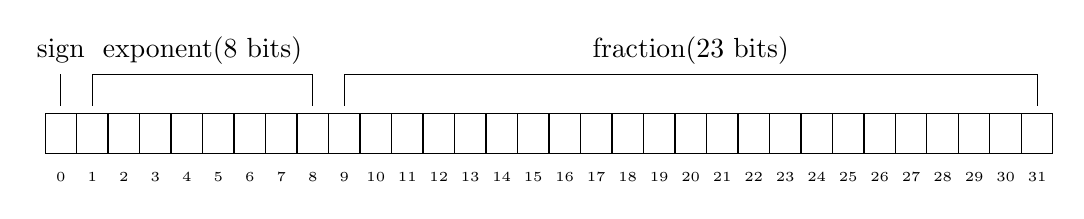
\begin{tikzpicture}[node distance=1.8cm]
  \foreach \x in {0, ..., 31}
  \draw (\x*0.4cm, 0) -- +(.4cm, 0) -- +(.4cm, 0.5cm) -- +(0, .5cm) --
  cycle;
  \draw (0.2cm, 0.6cm) -- (0.2cm, 1cm);
  \draw (0.6cm, 0.6cm) -- (0.6cm, 1cm) -- (3.4cm, 1cm) -- (3.4cm, 0.6cm);
  \draw (3.8cm, 0.6cm) -- (3.8cm, 1cm) -- (12.6cm, 1cm) -- (12.6cm, 0.6cm);
  \foreach \x in {31, ..., 0}
  \node at (\x*0.4cm, 0) [xshift=.2cm, yshift=-.3cm, align=center] {\tiny \x};
  \node at (0.2cm, 1.3cm) [align=center] {sign};
  \node at (2cm, 1.3cm) [align=center] {exponent(8 bits)};
  \node at (8.2cm, 1.3cm) [align=center] {fraction(23 bits)};
\end{tikzpicture}
\caption{32-bit floating-point numbers}
\label{fig:32-bit floating point numbers}
\end{center}
\end{figure}

Similarly in 64-bit floating point numbers we have 1 bit for sign, 11 bits for
exponent and 52 bits for fractional part. Clearly zero will be represented by
all sign and exponent bits having value 0 for them.

C also has concept of positive and negative infinities. Sign bit is 0 for
positive infinity and 1 for negative infinity. Fractional bits are 1 while
exponent bits are all 1.

Certain operations cause floating point exceptions like division from zero or
square rooting a negative number. Such exceptions are represented by NANs which
stands for ``not a number''. Sign for NaNs is similar i.e. 0 for positive and 1
for negative. Exponent bits are 1 and fractional part is anything but all 0s
because that represents positive infinity.

There is also four rounding modes which we will see later.

Now let us see a program to see how we can take input and print the floating
point numbers.

\begin{minted}[frame=single]{c}
#include <stdio.h>

int main()
{
  float f = 0.0;
  double d = 0.0;
  long double ld = 0.0;

  printf("Enter a float, double and long double separated by space:\n");
  scanf("%f %lf %Lf", &f, &d, &ld);

  printf("You entered %f %lf %Lf\n", f, d, ld);

  return 0;
}
\end{minted}

If you run this you might have following output:
\\\\\texttt{Enter a float, double and long double separated by space:\\
\textbf{3.4 5.6 7.8}\\
You entered 3.400000 5.600000 7.800000\\\\}
By default these print upto six significant digits but doubles have double
precision as we have studied. Now that we know basic types let us learn a bit
about input/output.

\section{Boolean Data Type}
A boolean type has only two values possible; \texttt{true} and
\texttt{false}. Fundamentally a boolean is an integer. 0 is considered as
\texttt{false} while all other are treated as \texttt{true} including negative
integers. \texttt{true} and \texttt{false} are macros (which we will see later)
which are defined in \texttt{<stdbool.h>} and they expand to 1 and 0
respectively. The type \texttt{bool} is a macro which expands to
\texttt{\_Bool}. Let us see a small program with booleans:

\begin{minted}[frame=single]{c}
#include <stdio.h>
#include <stdbool.h>

int main()
{
  bool bcpp      = 4;
  _Bool bc       = 5;
  bool True      = true;
  _Bool False    = false;
  bool bFalseCPP = -4;
  _Bool bFalseC  = -7;

  printf("%d %d %d %d %d %d\n", bcpp, bc, True, False, bFalseCPP, bFalseC);

  return 0;
}
\end{minted}

and the output is:
\\\\\texttt{1 1 1 0 1 1\\\\}
Note that \texttt{true} and \texttt{false} are keywords while \texttt{True} and
\texttt{False} are identifiers.

\section{Complex Type}
C99 introduced another type \texttt{complex}. As you may know a complex has two
parts real and imaginary. These parts of a complex individually are
floating-point numbers i.e. they can be represented by \texttt{float, double}
or \texttt{long double}. The header \texttt{<complex.h>} deals with complex
numbers and there are lots of useful functions to use and manipulate complex
numbers which are detailed in the reference. Let us see a simple example:

\begin{minted}[frame=single]{c}
#include <stdio.h>
#include <complex.h>

int main()
{
  double complex z = 4.0 + 3.0i;

  printf("Absolute value of z is %lf\n", cabs(z));

  double complex zConj = conj(z);
  printf("Imaghinary part of conjugate is now %lf\n", cimag(zConj));

  return 0;
}
\end{minted}

Since we have used \texttt{<complex.h>} we need to link math library to compile
this program so the compilation command would look like \texttt{\$gcc -o complex
complex.c -lm}. The \texttt{-lm} part is mandatory for compilation of this
program. Let us see the output:
\\\\\texttt{Absolute value of z is 5.000000\\
Imaginary part of conjugate is now -3.000000\\\\}
I have shown only two functions \texttt{cabs} and \texttt{cimag} but there are
a lot more and very useful functions available to do computations on complex
numbers. The way to declare a complex number is shown. It is a combination of
real part and imaginary part where imaginary part is coupled with $i$ which is
given by $i = \sqrt{-1}$. Here, \texttt{cabs} computes absolute value of
complex number which is given by $\sqrt{x^2 + y^2}$ where complex number is
given by $x + iy$. We will see rest of the functions in reference.

\section{Void and Enum}
The \texttt{void} type comprises an empty set of values; it is an incomplete
object type\footnote{An incomplete type is a type whose size is unknown.} that
cannot be completed. You cannot declare variables with type void. You cannot
declare an array of\texttt{void} type. Any declaration which requires size of
type to be known cannot have \texttt{void} as its type. However, we can declare
pointers of type \texttt{void} because pointers do not require size of type to
be known. For this reason \texttt{void} pointers are used as generic pointers
and is used to convert one type of pointers into another. It is a low-level
type and should be used sparingly. We will see examples of \texttt{void} type
later in the book.

Enum type is an integral type and is used as symbolic constants. An enumeration
is is a set of integers(values). You can do all operations of an enum on an
enumeration member which you can do on an integer. It starts from zero by
default and increments by one unless specifically specified. Given below is an
example of \texttt{enum} type.

\begin{minted}[frame=single]{c}
#include <stdio.h>

int main()
{
  typedef enum {zero, one, two} enum1;
  typedef enum {alpha=-5, beta, gamma, theta=4, delta, omega} enum2;

  printf("zero = %d, one = %d, two=%d\n", zero, one, two);
  printf("alpha = %d, beta = %d, gamma=%d, theta=%d, delta=%d, omega=%d\n", \
          alpha, beta, gamma, theta, delta, omega);

  return 0;
}
\end{minted}

and the output is:
\\\\\texttt{zero = 0, one = 1, two=2\\
alpha = -5, beta = -4, gamma=-3, tehta=4, delta=5, omega=6\\\\}

\section{Literals}
There are four categories of constants: character, integer, floating-point, and
enumeration constant. There are certain rules about constants. Commas and
spaces are not allowed except for character and string constants. Their range
cannot outgrow the range of there data type. For numeric type of constants they
can have a leading (-)minus sign.

Given below is an example of integer constants:

\begin{minted}[frame=single]{c}
#include <stdio.h>

int main()
{
  int decimal = 7;
  int octal = 06;
  int hex = 0xb;

  printf("%d %o %x\n", decimal, octal, hex);

  return 0;
}
\end{minted}

and the output is:
\\\\\texttt{7 6 b\\\\}
As you can see there are three different categories for integer constants:
decimal constants (base 10), octal constants (base 8) and hexadecimal constants
(base 16). Also, you must have noticed how a zero is prefixed before octal type
and a zero and x for hexadecimal type. The \texttt{\%d} format specifier is
already known to you for signed decimals. However, now you know two more
\texttt{\%o} and \texttt{\%x} for unsigned octal and unsigned hexadecimal
respectively. For unsigned integer it is \texttt{\%u}. There is one more format
specifier which you may encounter for signed decimal and that is
\texttt{\%i}. Note that there is nothing for binary constants.

A floating-point constant is a base-10 number that contains either decimal
point or exponent or both. Given below is an example of floating-point
constants:

\begin{minted}[frame=single]{c}
#include <stdio.h>

int main()
{
  float f = 7.5384589234;
  double d = 13.89457883453857823;
  long double ld = 759.8263478234729;

  printf("%f %lf %Lf\n", f, d, ld);

  return 0;
}
\end{minted}

and the output is:
\\\\\texttt{7.538459 13.894579 759.826348\\\\}
For example 123456 can be written as one of 1.23456e5, 1.23456e+5, 1.23456E5,
.123456e6, 12.3456E+4 etc. The expoenent is integer and it cannot be
floating-point number.

A character constant is a single character enclosed in apostrophes. Some
examples of a character constants are \texttt{`A', `T', `)', `?'. ` '}. Commas
and blanks are allowed as character constants in apostrophes. The character
constants are fundamentally integers and all arithmetic operations can be
performed over them. These values depend on the character set of the computer
in use. However, in this book we are concerned about ASCII character set.

\begin{minted}[frame=single]{c}
// Character constants
// Description: Demo of character constants

#include <stdio.h>

int main()
{
  char c = 'S';
  char* str ="Shiv S. Dayal";

  printf("%c %s\n", c, str);

  return 0;
}
\end{minted}

and the output is:
\\\\\texttt{S Shiv S. Dayal\\\\}
Also, the string is a character pointer that is it can point to memory location
where a character is stored. In this case the string is stored in an area of
memory called stack. When memory is allocated the compiler knows how much has
been allocated. For string there is something called null character represented
by \texttt{\textbackslash{} 0} which is used to terminate string. By using this mechanism
the program knows where the string is terminating. It is treated in next
section as well.A very interesting thing to be noted is char is considered to
be an integral type. It is allowed to perform addition etc on char type. Till
now you have learnt many format specifiers and have seen they all start with
\texttt{\%}. Think how will you print \texttt{\%} on stdout. It is printed like
\texttt{\%\%}.  C program have got something called ASCII table which is a
7-bit character table values ranging from0 to 127. There is also something
called escape sequences and it is worth to have a look at them.

\section{Escape Sequences}
There are certain characters which are not on keyboard and are not displayed in
the form on printing characters. Some of these are expressed using
\textit{escape sequences}. An escape sequence always begins with a backslash
and is followed by on or more characters. Given below is the table of escape
sequences:

\begin{table}[H]
\begin{center}
\caption{Escape Sequences}
\begin{longtable}{lcc}
\textbf{Character}&\textbf{Escape Sequence}&\textbf{ASCII Value}\\
bell (alert)&$\backslash$a&007\\
backspace&$\backslash$b&008\\
horizontal t&$\backslash$t&009\\
vertical tab&$\backslash$v&011\\
newline (line feed)&$\backslash$n&010\\
form feed&$\backslash$f&012\\
carriage return&$\backslash$r&013\\
quotation mark(")&$\backslash$"&034\\
apostrophe(')&$\backslash$'&039\\
question mark(?)&$\backslash$?&063\\
backslask ($\backslash$)&$\backslash\backslash$&092\\
null&$\backslash$0&000
\end{longtable}
\end{center}
\end{table}

Now we will talk about all these one by one. \texttt{\textbackslash{} 0} which
is also known as \texttt{NULL} is the string terminating character, as said
previously, and must be present in string for it to terminate. For example, in
our character constant program the str string is \texttt{"Shiv S. Dayal"}. So
how many characters are there 13? Wrong 14! The NULL character is hidden. Even
if we say \texttt{str="";} then it will contain one character and that is this
\texttt{NULL}. Most string related C functions rely on this presence of
\texttt{NULL} and causes a lot of mess because of this if missing. The bell
escape sequence if for a bell from CPU. Let us write a program and see it in
effect.

\begin{minted}[frame=single]{c}
// Bell Program
// Description: Demo of bell escape sequence

#include <stdio.h>

int main()
{
  printf("hello\a");

  getchar();

  return 0;
}
\end{minted}

The output of this program will be \texttt{hello} on \texttt{stdout} and an
audible or visible bell as per settings of your shell. Notice the
\texttt{getchar()} function which waits for input and reads a character from
\texttt{stdin}. Next is backspace escape sequence. Let us see a program for its
demo as well:

\begin{minted}[frame=single]{c}
// Backspace Program
// Description: Demo of backspace escape sequence

#include <stdio.h>

int main()
{
  printf("h\b*e\b*l\b*l\b*o\b*\n");
  printf("\b");

  getchar();

  return 0;
}
\end{minted}

and the output is:
\\\\\texttt{*****}\\\\
It is \texttt{hello} replaced by \texttt{*}s. A minor modification in this
program to replace the character as soon as key is pressed by some other
character will turn it into a password program. Backspace escape sequence means
when it is encountered the cursor moves to the previous position on the line in
context. If active position of cursor is initial position then C99 standard
does not specify the behavior of display device. However, the behavior on my
system is that cursor remains at initial position. Check out on yours. The
second \texttt{printf} function determines this behavior.

Next we are going to deal with newline and horizontal tab escape sequences
together as combined together they are used to format output in a beautiful
fashion. The program is listed below:

\begin{minted}[frame=single]{c}
// Newline and Horizontal tab program Program
// Description: Demo of newline and horizontal tab escape sequence

#include <stdio.h>

int main()
{
  printf("Before tab\tAftertab\n");
  printf("\nAfter newline\n");

  getchar();

  return 0;
}
\end{minted}

and the output is:
\\\\\texttt{Before tab~~~~Aftertab}\\\\
\texttt{After newline}\\\\
Here I leave you to experiment with other escape sequences. Feel free to
explore them. Try various combinations; let your creative juices flow.
